\documentclass[12pt,letterpaper]{article}

\usepackage[spanish,es-tabla,es-nodecimaldot]{babel}
\usepackage{amsmath}
\usepackage[utf8]{inputenc}
\usepackage[T1]{fontenc}
\usepackage{lmodern}
\usepackage{graphicx}
\usepackage{listings}
\usepackage{anysize} 
\usepackage{fancyhdr}
\usepackage{amsmath}
\usepackage{pdfpages}
\usepackage{graphics}
\usepackage{capt-of}
\usepackage{tabularx}
\usepackage[colorlinks=true,plainpages=true,citecolor=blue,linkcolor=blue]{hyperref}

\marginsize{2cm}{2cm}{2cm}{2cm}
\pagestyle{fancy}
\fancyhf{Redes de Telecomunicaciones}
\fancyhead[L]{\footnotesize UPIITA-IPN} 
\fancyhead[R]{\footnotesize 4TV2} 
\fancyfoot[R]{\footnotesize Memoría técnica}
\fancyfoot[C]{\thepage}
\fancyfoot[L]{\footnotesize La Costeña} 

\renewcommand{\footrulewidth}{0.4pt}
\renewcommand{\spanishtablename}{Tabla}
\renewcommand{\labelitemii}{$\star$}

\begin{document}

\includepdf[pages={1}]{portada2}

\newpage
\tableofcontents
\listoffigures
\listoftables

\newpage
\section{Poligonal}
\subsection{Coordenadas}
\begin{itemize}
    \item \textbf{La Costeña corporativo:} $N 19.44 \ W 99.20$
    \item \textbf{Central Telmex Polanco:} $N 19.43 \ W 99.20$
    \item \textbf{Centro de datos:} $N 19.41 \ W 99.09$
    \item \textbf{Central Telmex Moctezuma:} $N 19.42 \ W 99.09$
    \item \textbf{MCM Telecom:} $N 19.43 \ W 99.21$
\end{itemize}

\newpage
\section{Perfil de elevación }

\newpage
\section{Ruta}
\subsection{Ruta principal y alternativa}
Ruta principal tomando la mayor parte del trayecto por metro.
\begin{figure}[ht]
    \centering
    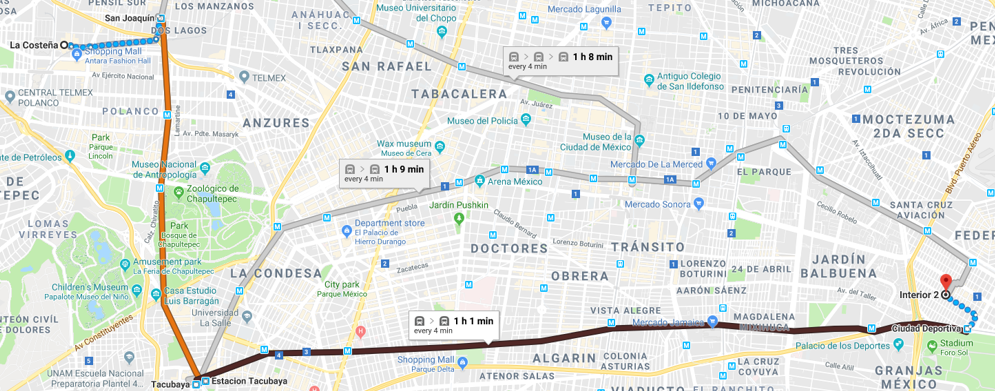
\includegraphics[width=.9\textwidth]{f2.png}
    \caption{Ruta principala a escala.}
\end{figure}

La ruta alternativa cuenta con tramo principal por avenidas 
vehiculares.
\begin{figure}[ht]
    \centering
    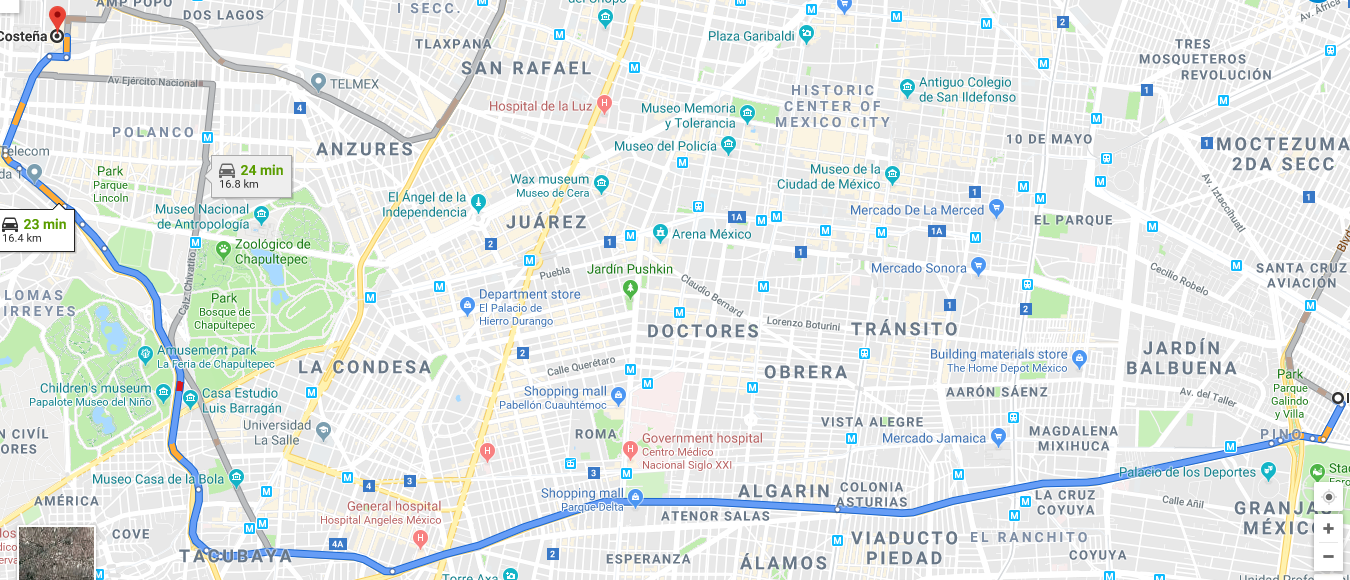
\includegraphics[width=.9\textwidth]{f3.png}
    \caption{Ruta alternativa a escala.}
\end{figure}

\newpage
\subsection{Salida de corporativo}
Se propone que la salida de la salida de la fibra sea por el 
sótano que es donde se encuentra el site del edificio.
\begin{figure}[ht]
    \centering
    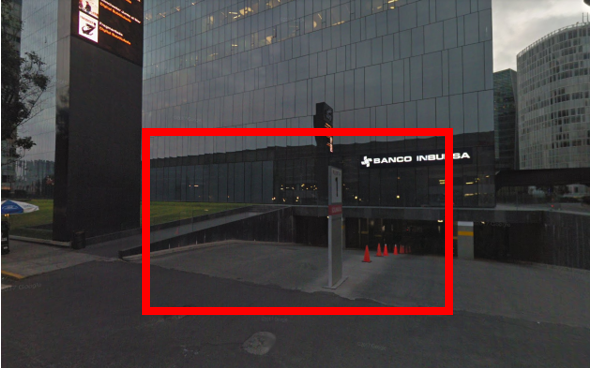
\includegraphics[width=.6\textwidth]{f0.png}
    \caption{Salida de corporativo.}
\end{figure}

Una vez fuera se tomará el siguiente registro para llevarlo por 
subsuelo hasta el metro.
\begin{figure}[ht]
    \centering
    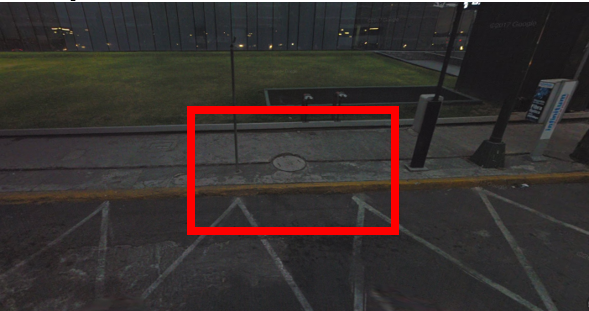
\includegraphics[width=.7\textwidth]{f1.png}
    \caption{Registro donde iniciar el recorrido.}
\end{figure}

\newpage
\subsection{Puntos críticos: Ruta principal}
\subsubsection{Primer tramo}
A continuación se muestra el primer tramo del recorrido. Este 
tramo es del corporativo al metro.
\begin{figure}[ht]
    \centering
    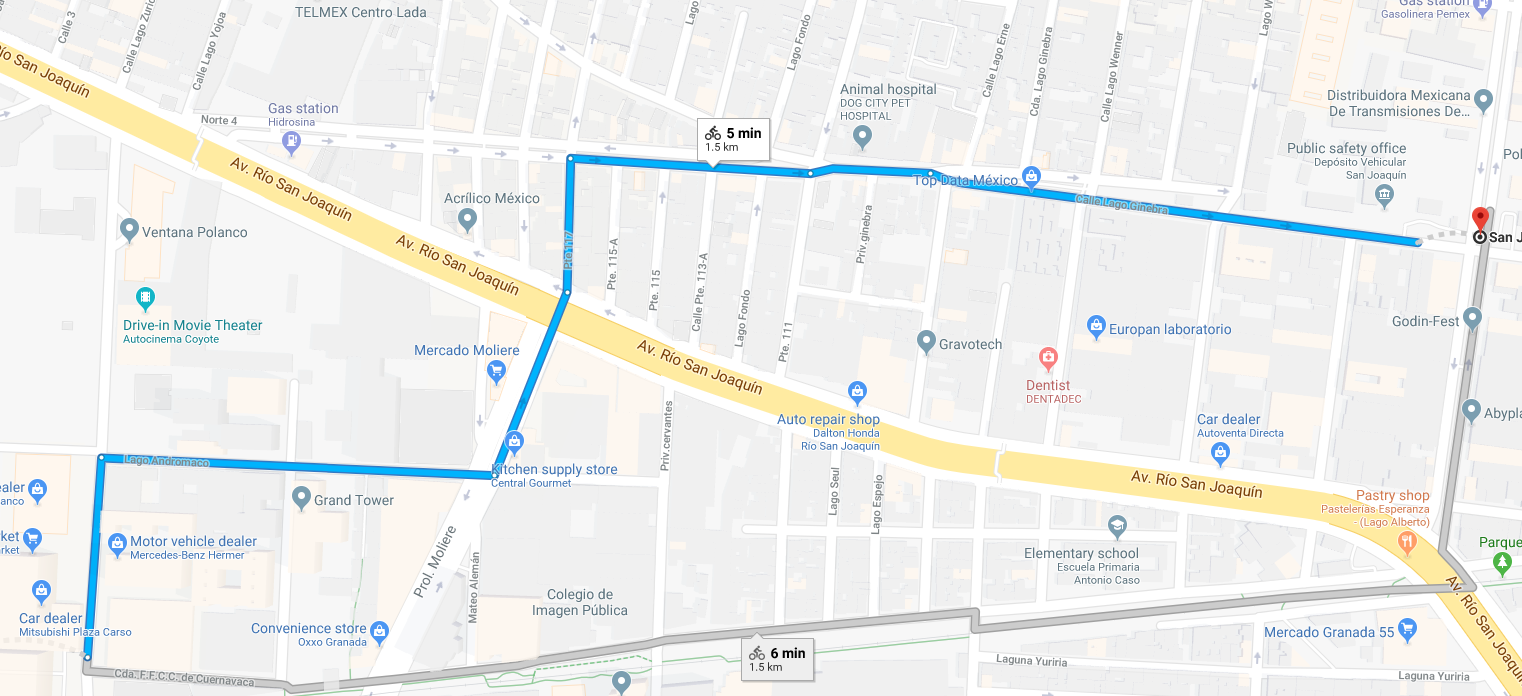
\includegraphics[width=.8\textwidth]{f5.png}
    \caption{Vista aerea primer tramo.}
\end{figure}

El primer punto crítico se encuentra en el puente para cruzar la 
avenida Río San Joaquín.
\begin{figure}[ht]
    \centering
    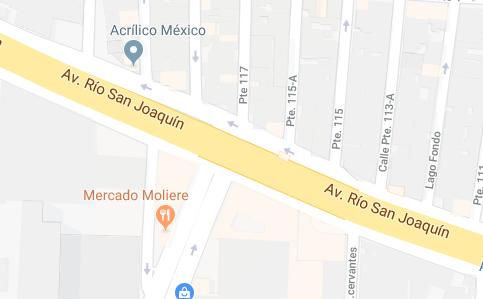
\includegraphics[width=.6\textwidth]{f4.png}
    \caption{Vista aerea punto crítico.}
\end{figure}

Para sortear este obstáculo se tendrá que utilizar un tendido aéreo 
para posteriormente volver a introducirlo en el subsuelo.
\begin{figure}[ht]
    \centering
    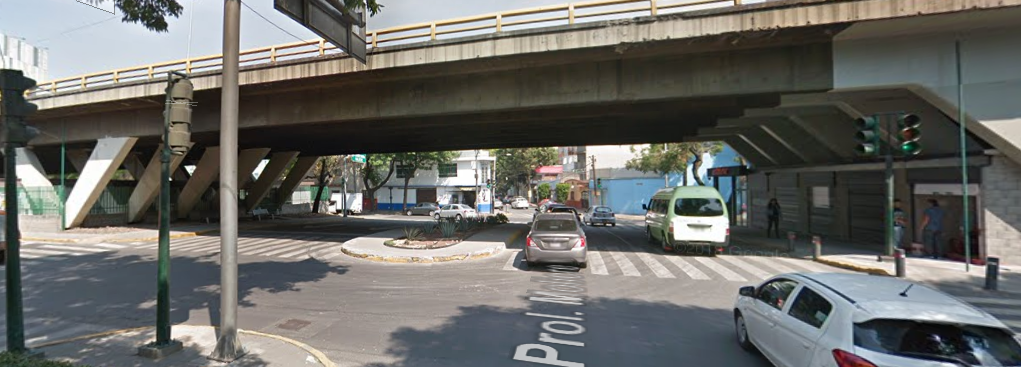
\includegraphics[width=1\textwidth]{f6.png}
    \caption{Punto crítico.}
\end{figure}

\subsubsection{Segundo tramo}
El segundo tramo consta de todo el recorrido en metro. En este 
tramo se cuenta con un punto crítico es cúal es el cambio de lineas 
9 y 4.
\begin{figure}[ht]
    \centering
    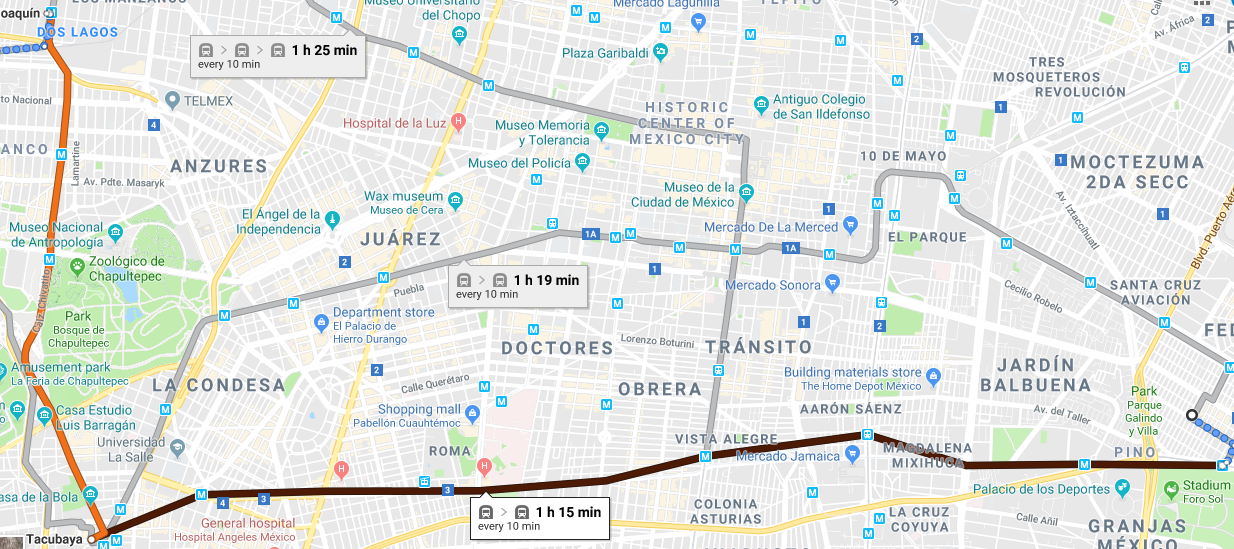
\includegraphics[width=1\textwidth]{f7.png}
    \caption{Vista aerea segundo tramo.}
\end{figure}
\\
El punto crítico de este tramo se encuentra en el cambio de lineas.
\begin{figure}[ht]
    \centering
    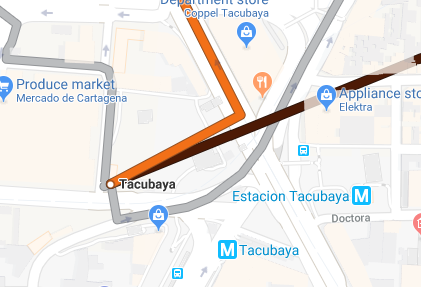
\includegraphics[width=.5\textwidth]{f8.png}
    \caption{Punto crítico segundo tramo.}
\end{figure}

\newpage
\subsubsection{Tercer tramo}
El tercer tramo del recorrido consta de la salida del metro hasta
el centro de datos.
\begin{figure}[ht]
    \centering
    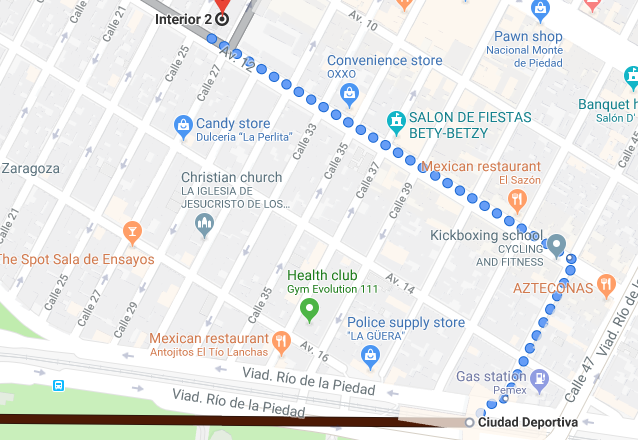
\includegraphics[width=.5\textwidth]{f9.png}
    \caption{Punto crítico segundo tramo.}
\end{figure}

En este tramo el punto crítico se encuentra a la salida del metro 
para mandarlo hacía el corporativo por tendido aéreo.
\begin{figure}[ht]
    \centering
    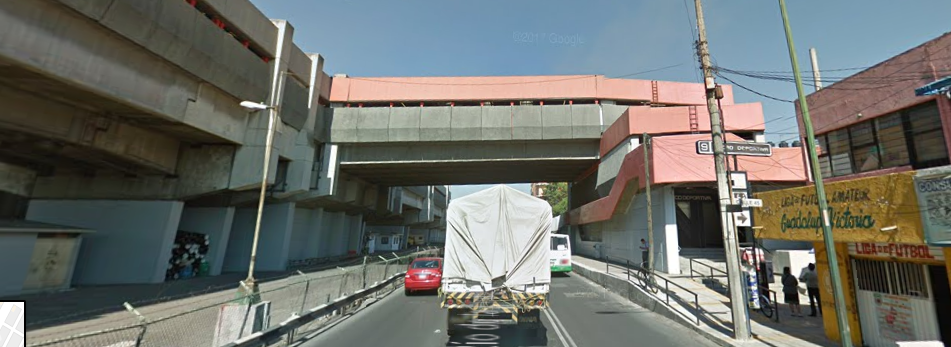
\includegraphics[width=.9\textwidth]{f10.png}
    \caption{Punto crítico segundo tramo.}
\end{figure}

\newpage
\subsection{Estimación}
\subsubsection{Ruta principal}
\begin{itemize}
    \item Longitud de recorrido: 15.5 $km$
    \item Longitud redundante: $15.5*.20\%=3.1km$
    \item Longitud total: 18.6 $km$
\end{itemize}

\subsubsection{Ruta secundaria}
\begin{itemize}
    \item Longitud de recorrido: 16.5 $km$
    \item Longitud redundante: $16.5*.20\%=3.3km$
    \item Longitud total: 19.8 $km$ 
\end{itemize}

\newpage
\section{Ductos}
\subsection{Antecedente}
Hoy en día, los cables de fibra óptica casi siempre se instalan en los sistemas de 
conductos existentes. Normalmente debido a que el sistema de conducto existente está 
sobrellenado y, por otro lado, una nueva construcción de sistema de conducto es costosa, 
esos dos factores constituyen un problema.
\\ \\
El sistema de microconducto y multuductos y las redes de microcable resuelven el problema 
de forma integral. Se presentan como un microducto único o como multiductos, es decir, un 
conjunto o haces de microductos envueltos en una camisa fina exterior o bien dentro de un 
conducto de diámetro 32,40 ó 50 mm.
\\ \\
Los microductos directos enterrados y de interior se instalan directamente en el suelo o 
dentro de los edificios. Los multiductos también se instalan dentro de un sistema de 
conductos existentes aumentando su capacidad o directamente enterrados en el suelo.

\subsubsection{Tendido subterráneo}
La instalación de fibra óptica que ocurre cuando el cable de fibra óptica se instala bajo 
tierra en tuberías, o conductos, se conoce como construcción subterránea. En este caso, los 
cables de fibra se entierran en una zanja. La profundidad de los cables subterráneos varía 
según muchos factores; sin embargo, normalmente está entre 12 y 36 pulgadas por debajo del 
nivel de la superficie. En las zonas más frías, los cables de fibra normalmente se entierran 
por debajo de la línea de congelación para evitar que se dañen. Muchas compañías y 
contratistas construyen conductos adicionales a lo largo de la ruta, para prevenir futuras 
excavaciones para instalaciones de cables adicionales.
\begin{figure}[ht]
    \centering
    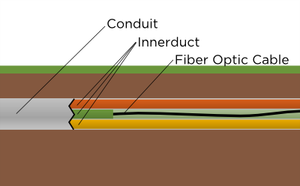
\includegraphics[width=.5\textwidth]{f11.png}
    \caption{Tendido subterráneo.}
\end{figure}

\subsubsection{Tendido aéreo}
La construcción de fibra aérea es el proceso por el cual se instala el cable de fibra 
óptica a lo largo de una línea de postes de servicios públicos. Al colocar la fibra, se 
necesita un filamento de soporte además del cable. Algunas fibras aéreas están 
preenganchadas a una hebra de soporte, lo que hace que la colocación sea menos compleja. 
Los filamentos también pueden ser colocados a lo largo de la ruta primero, con la fibra 
tirada y anclada al filamento de soporte después. El amarre es el proceso de asegurar el 
cable de fibra al filamento de soporte a través del alambre de amarre. Cuando se coloca 
un cable en un poste, la distancia de separación requerida varía dependiendo del tipo de 
cable o equipo. Estos requisitos a menudo son establecidos por estándares locales, 
estatales y nacionales.
\begin{figure}[ht]
    \centering
    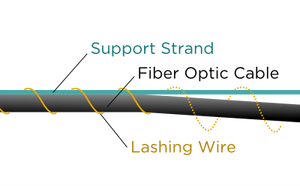
\includegraphics[width=.5\textwidth]{f12.png}
    \caption{Tendido aéreo.}
\end{figure}

\subsection{Ductos para ruta}
\subsubsection{Material para ruta subterránea e interiores}
\textbf{Ducto de protección}
\\
De la compañia Pestan se elegió el siguiente ducto.
\begin{figure}[ht]
    \centering
    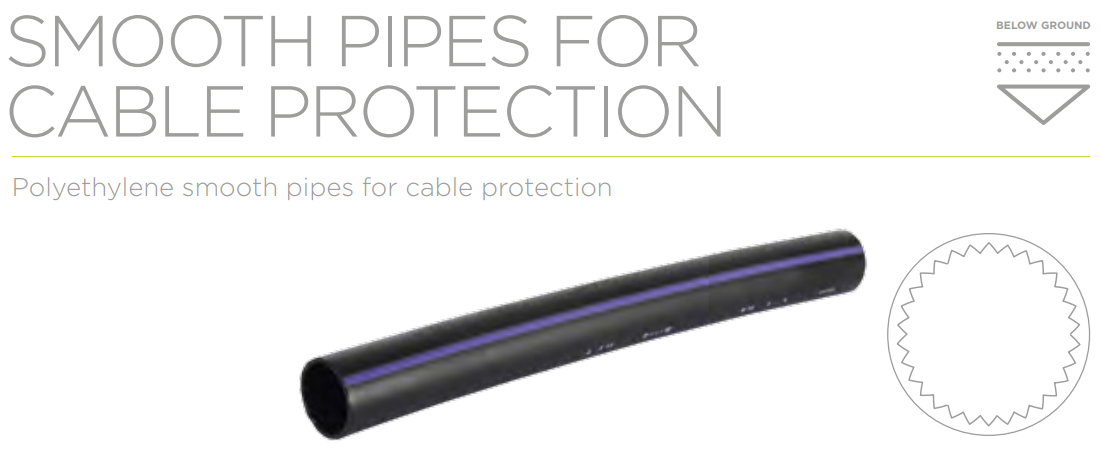
\includegraphics[width=.5\textwidth]{f13.png}
    \caption{Ducto de protección.}
\end{figure}
\\
Esta opción cuenta con los siguientes diámetros, así como opciones personalizadas.
\begin{figure}[ht]
    \centering
    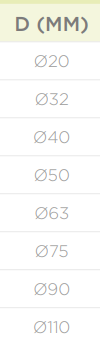
\includegraphics[width=.1\textwidth]{f14.png}
    \caption{Ducto de protección.}
\end{figure}

\subsubsection{Material para ruta aérea}
De la compañia blue diamond industries se opto por el siguiente producto.
\begin{figure}[ht]
    \centering
    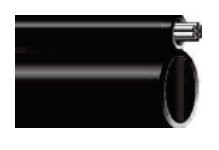
\includegraphics[width=.5\textwidth]{f15.png}
    \caption{Ducto de protección.}
\end{figure}
\\
\textbf{Descripción}
\\
El HDPE es un conducto aéreo utilizado en cruces aéreos, de carreteras o de agua 
y en aplicaciones de edificio a edificio. Blue Diamond ofrece conductos aéreos en 
dimensiones de 1-1/4" de diámetro True SDR 9 con un cordón galvanizado de 1/4".

\newpage
\section{Fibras}

\newpage
\section{Arquitectura}
\begin{figure}[ht]
    \centering
    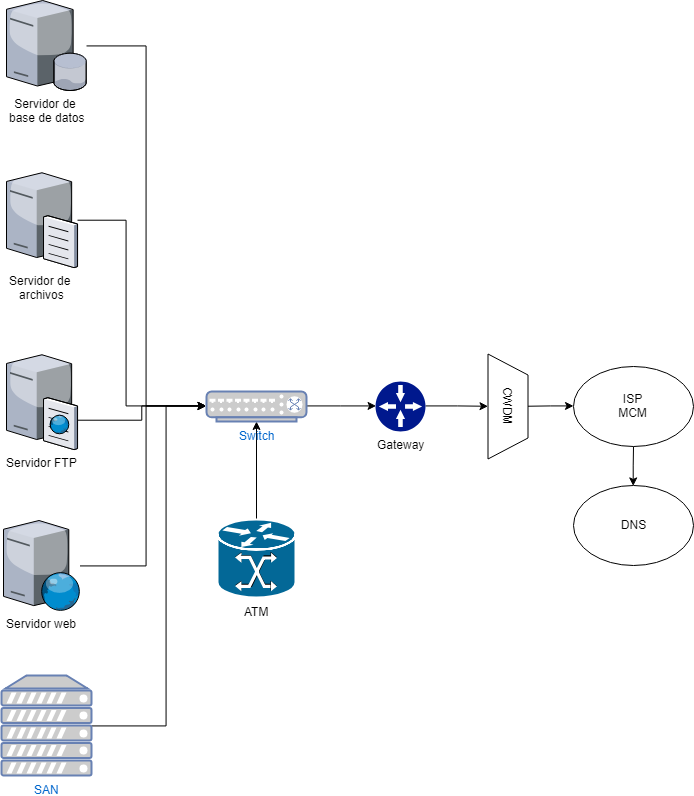
\includegraphics[width=.75\textwidth]{f16.png}
    \caption{Arquitectura.}
\end{figure}

\newpage
\section{E-commerce}


\newpage
\begin{thebibliography}{20}
    \bibitem{anchobanda}
    https://sunesysllc.wordpress.com/2014/05/20/aerial-vs-underground-fiber/

    \bibitem{radiacion}
    https://pestan.net/en/hdpe-cable-protection-pipes/
    
    \bibitem{polarizacion}
    %https://www.bdiky.com/siteadmin/includes/javascript/third_party/kcfinder/upload/files/Fig\%208\%20Data\%20Sheet\%205-18.pdf

    \bibitem{haz}
    W. L. Stutzman and G. A. Theile, Antenna theory and design. John Wiley and Sons, Inc., 1998.
\end{thebibliography}

\end{document}